\section{Transition systems}
\label{sec:ordinary-transition-systems}
    
    %Transition systems are a commonly used and understood model of computation. They provide the basic operational semantics for Milner’s Calculus of Communicating Systems (CCS) and often underlie other approaches, such as that of Hoare’s Communicating Sequential Processes (CSP). The constructions on transition systems used in such methods can frequently be seen as universal in a category of transition systems, where the morphisms can be understood as expressing the partial simulation (or refinement) of one process by another. By “abstract nonsense” the universal properties will characterise the constructions to within isomorphism. More strikingly, the same universal properties will apply in the case of other models like Petri nets or event structures, which are seemingly very different in nature.
    
    Transition systems are well established semantic models for both sequential and concurrent systems. A transition system can be viewed as a directed graph, called a state transition graph, whose vertices are states and edges are transitions between states. We may consider a transition system, as shown in Figure \ref{fig:transition-system}, where we have four states $s_{1}$, $s_{2}$, $s_{3}$, and $s_{4}$, for example, representing a program changing a value of a variable at different times of its execution. We also have four transitions, two of which are labeled $a$ and another two which are labeled $b$. We can also have the same label $a$ for both events, giving rise to the notion of \emph{autoconcurrency}. These four transitions, represent two instructions of a program that change the state of the machine from the source of its arrow to its corresponding target. This is formalized by using a transition relation. We will refer to this transition system as the \emph{interleaving square}, similar to what has been done by Pratt \cite{Pratt00Sculptures} and van Glabbeek \cite{Glabbeek06HDA}. We will use the same notation and definitions as Winskel and Nielsen in \cite{winskel95modelsCategory}.
    %We will use the same notation as in \cite{winskel95modelsCategory}.
    
    %     Transition systems are a well established semantic model for both sequential and concurrent systems. A classic form of transition systems is state transition graphs, which are simply directed graphs. We may consider a transition system, as shown in Figure \ref{fig:transition-system}, where we have four states $s_{1}$, $s_{2}$, $s_{3}$ and $s_{4}$ representing, for example, the value of a program at different times of its execution. We have also four transitions, two $a$ and two $b$ which are two instructions of a program that changes the state of the machine from the source of its arrow to its corresponding target. This is formalized by using a transition relation. We will refer to this transition system as the \emph{interleaving square}, similar to what has been done in \cite{Pratt00Sculptures} and \cite{Glabbeek06HDA}. We will use the same notation as in \cite{winskel95modelsCategory}.
    
    %As shown in Figure \ref{fig:transition-system}, we may picture a transition system as such. We have seven states $s_{1},...,s_{7}$ representing, for example, the value of a program at different times of its execution. We have also ten transitions, two $a$, two $b$, two $e_{4}$, $e_{3}$, $e_{5}$, $e_{6}$ and $e_{7}$ which are seven instructions of a program that changes the state of the machine from the source of its corresponding arrow to its target. This is formalized by using a transition relation. We will use the same notation as in \cite{winskel95modelsCategory}.

    %Transition systems are one of the most known models of computation. They are nothing but state transition graphs and can be pictured as such. Look for instance at Figure \ref{fig:transition-system}. We have five states $\alpha, \beta, \delta, \epsilon$ and $\gamma$ representing, for example, the value of the variables of a program at different times of its execution. We have also six transitions, two $a$s, two $b$s, $c$ and $d$. $a, b, c$ and $d$ are four instructions of a program which change the state of the machine from the source of its corresponding arrow to its target.

    \begin{figure}[ht]
        \centering
        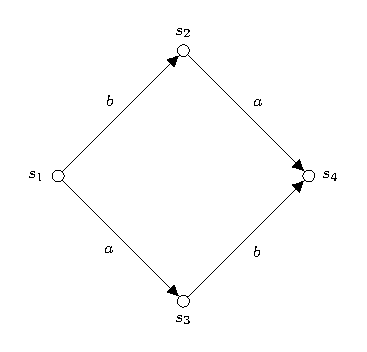
\includegraphics[scale=1.3]{Figures/2.Models-for-concurrency/transition-system.pdf}
        \captionof{figure}[A transition system.]{A transition system with four states, $s_{1}, s_{2}, s_{3}$, and $s_{4}$, and four transitions, two of which are labeled $a$ and the other two are labeled $b$. These four transitions present the interleaving of two instructions. The interleaving is namely the permutation of all possible executions of these two instructions. This transition system is called the interleaving square because of the way the interleaving of two instructions form a square.}
        \label{fig:transition-system}
      
    \end{figure}
    
    %This is generally formalized using a transition relation. We use the same notation as in \cite{winskel95modelsCategory}.
    
    \begin{definition}[Transition system \cite{winskel95modelsCategory}]\label{def:transition-system}
        A transition system is a structure ($\mathcal{S}, i, \mathcal{L}, Tran$) where,
        \begin{itemize}
            \item $\mathcal{S}$ is a set of states with initial state i,
            \item $\mathcal{L}$ is a set of labels, and
            \item $Tran \subseteq \mathcal{S} \times \mathcal{L} \times \mathcal{S}$ is the transition relation
        \end{itemize}
    \end{definition}
    
    We will write $s \xrightarrow{a} s'$ to indicate  that $(s,a,s') \in Tran$.
    
    Morphisms between transition systems often describe the relationships between processes. These kind of relations are described by Winskel and Nielsen in \cite{winskel95modelsCategory}, where one process may be a component of another or perhaps one process may refine another process. By defining morphisms as simulations between transition systems, we are able to describe the relationship between processes. For example, a simulation is where a transition system $\mathcal{T}$ simulates a transition system $\mathcal{T}^{'}$, meaning that when $\mathcal{T}^{'}$ can execute some action $a$ then there must exists an $a$ in $\mathcal{T}$ that can be executed.
    
   % Morphisms between transition systems often describe the behavior between processes. Processes may arise in relation to other processes. As an example, from the Introduction of \cite{winskel95modelsCategory}, one processes may refine another, or perhaps one process is a component of another. By defining morphisms as the behavior between transition systems, we may consider morphisms to be a simulation. If we consider a transition system $T$ simulates a transition system $T'$ , then it means that when $T'$ can execute some action $a$, then $T$ can execute $a$ as well in some related context. 
    %We introduce morphisms of transition systems as shown in \cite{winskel95modelsCategory}.
    
    \begin{definition}[Morphism of transition systems \cite{winskel95modelsCategory}]\label{def:morphism-of-transition-system}
        A morphism from one transition system, $\mathcal{T}$, to another, $\mathcal{T}^{'}$ , will be a pair $(\sigma, \lambda)$ in which
        \begin{itemize}
            \item $\sigma$ is a function from the states of $\mathcal{T}$ to those of $\mathcal{T}^{'}$ .
            \item $\lambda$ is a partial function from the labels of $\mathcal{T}$ to those of $\mathcal{T}^{'}$ such that for any transition $s \xrightarrow{a} s'$ of $\mathcal{T}$ if $\lambda(a)$ is defined, then $\sigma(s) \xrightarrow{\lambda(a)} \sigma(s')$ is a transition of $\mathcal{T}^{'}$ ; otherwise, if $\lambda(a)$ is undefined, then $\sigma(s) = \sigma(s')$.
        \end{itemize}
    \end{definition}
    
    In our notation, we have used $\mathcal{L}$ to stand for the set of labels for events, as well as to stand for the actual set of those events. However, sometimes it might be useful to make a distinction between the events themselves and to explicitly give a labeling as a function. For instance, this is important when treating \emph{relabeling} which leads to categorical fibrational situations \cite{winskel95modelsCategory}. To make the distinction between labels of events and the actual events clearer, we will replace $\mathcal{L}$ with $E$ and refer to its elements as \emph{events}.
    
    \begin{definition}[Labeled transition system \cite{winskel95modelsCategory}]\label{def:labeled-transition-system}
        A \emph{labeled} transition system consists of a transition system $\mathcal{T}$ = ($\mathcal{S}, i, E, Tran$) together with a set $\mathcal{L}$ of labels, and a function $l: E \rightarrow \mathcal{L}$. We denote it by ($\mathcal{T}$, $\mathcal{L}$, $l$).
    \end{definition}
    
    \begin{definition}[Morphism of labeled transition systems \cite{winskel95modelsCategory}]\label{def:morphisms-labeled-transition-system}
        A morphism, ($\sigma,\tau, \lambda$) : ($\mathcal{T}$, $\mathcal{L}$, $l$) $\rightarrow$ ($\mathcal{T}^{'}$, $\mathcal{L}^{'}$, $l^{'}$) between labeled transition systems consists of a morphism ($\sigma, \tau$) : $\mathcal{T} \rightarrow \mathcal{T}^{'}$ between the underlying transition systems together with a partial function $\lambda : \mathcal{L} \rightarrow \mathcal{L}^{'}$ such that $l' \circ \tau = \lambda \circ l$.
    \end{definition}

    %We will extend on the notion of transition systems to consider "\emph{idle}" transitions as shown in Figure \ref{fig:idle-transition-system}. It is convenient to introduce "\emph{idle}" transitions, associated with any state. Idle transitions help simplify the definition of morphisms between transition systems. By adopting the notation in \cite{winskel95modelsCategory}, it allows us to view the partial function from a set $\mathcal{L}$ to a set $\mathcal{L}^{'}$ as a total function $\lambda : \mathcal{L} \rightarrow \mathcal{L}^{'} \cup \{*\}$, where we will follow the notation that $*$ is a distinguished element standing for "\emph{undefined}". As done by Winskel in \cite{winskel95modelsCategory}, we will reflect the representation of $*$ in our notation $\lambda : \mathcal{L} \rightarrow_{*} \mathcal{L}^{'}$, for a partial function $\lambda$ from $\mathcal{L}$  to $\mathcal{L}^{'}$. 
    
    %\begin{figure}[ht]
    %    \centering
    %    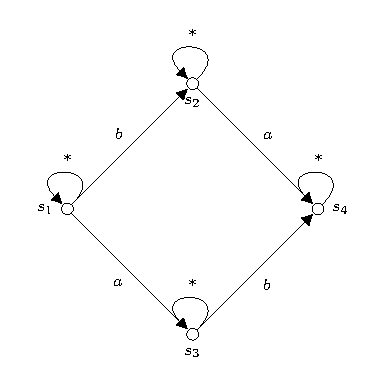
\includegraphics[scale=1.3]{Figures/2.Models-for-concurrency/idle-transition-system.pdf}
    %    \captionof{figure}[An idle transition system.]{A transition system with four states, $s_{1}, s_{2}, s_{3}$, and $s_{4}$, and eight transitions, two of which are labeled $a$, another two which are labeled $b$ and the remaining are loops labeled $*$. The paths with $a$ and $b$ represent the interleaving of two instructions. The interleaving is namely the permutation of all possible executions of these two instructions. While, transitions labelled $*$ refer to the possible inaction of a transition system.}
    %    \label{fig:idle-transition-system}
    %\end{figure}
    
    %This representation will also be reflected in our notation $\lambda : \mathcal{L} \rightarrow_{*} \mathcal{L}^{'}$, for a partial function $\lambda$ from $\mathcal{L}$  to $\mathcal{L}^{'}$. 
    %We define idle transition systems as in \cite{winskel95modelsCategory}.
    
    %\begin{definition}[Idle transition systems \cite{winskel95modelsCategory}]\label{def:idle-transition-system}
    %    Let $\mathcal{T}$ = ($\mathcal{S}, i, \mathcal{L}, Tran$) be a transition system. An idle transition of $\mathcal{T}$ consists of ($s, *, s$) and $s \in \mathcal{S}$ such that
    %    \begin{center}
    %        $Tran_{*} = Tran \cup \{(s,*,s)\ |\ s \in \mathcal{S}\}$.
    %    \end{center}
    %\end{definition}
    
    %We may also define morphisms between idle transition systems as follows:
    
    %\begin{definition}[Morphisms of idle transition systems \cite{winskel95modelsCategory}]\label{def:morphisms-of-idle-transition-system}
    %    Let $\mathcal{T}$ = ($\mathcal{S}, i, \mathcal{L}, Tran$) and $\mathcal{T}^{'}$ = ($\mathcal{S}^{'}, i^{'}, \mathcal{L}^{'}, Tran^{'}$) be transition systems. A morphism $f : \mathcal{T} \rightarrow \mathcal{T}^{'}$ is a pair $f = (\sigma, \lambda)$ where
    %    \begin{itemize}
    %        \item $\sigma : \mathcal{S} \rightarrow \mathcal{S}^{'}$
    %        \item $\lambda : \mathcal{L} \rightarrow \mathcal{L}^{'}$ are such that $\sigma(i)$ = $i'$ and $(s,a,s') \in Tran \Rightarrow (\sigma(s),\lambda(a),\sigma(s')) \in Tran^{'}_{*}$.
    %    \end{itemize}
    %\end{definition}
    
    %If a transition with label $a$ in $\mathcal{T}$ is undefined, then we want a transition with label $\lambda(a)$ in $\mathcal{T}^{'}$ to also be undefined. We will consider this as a transition representing inaction. With the introduction of idle transitions, morphisms on transition systems can be described as preserving transitions and the initial state. Lastly, we will also stress, as done in \cite{winskel95modelsCategory}, that an idle transition ($s, *, s$) represents inaction, and is to be distinguished from the action expressed by a transition ($s, a, s$) for a label \emph{a}. From now on, when referring to transition systems we mean idle transition systems with the extension of morphisms of transition systems considering idle transitions.
    
    We write $\allTS$ for the category of transition systems. Also, we name $\allTS_{E}$ its subcategory where we restrict to transition systems labeled on an alphabet $E$. The alphabet $E$ can be considered the same as the set of events $E$. The notion of transition systems and of morphisms between them is clearly related to directed graphs, labeled directed graphs, and labeled transition systems, but we will need to consider labeled cubical sets, which we will not do here. However, we will introduce precubical sets\footnote{In topology, the difference between cubical and precubical sets are similar to that of simplicial and presimplicial sets. The differences are subtle and will not be considered here. The distinction between cubical and precubical sets is presented in \cite{Goubault95PhDThesis}.} in Section \ref{sec:higher-dimensional-automata}.
    
    %%%% Difference! %%%%%
    %there's, unfortunately, some confusion of terminology in the literature. Here's the one I consider the most standard:

    %A precubical set is a set of things of different dimensions together with face maps \delta_i^0, \delta_i^1 from X_n to X_{n-1}, for i from 1 to n. This is what we usually use for HDA (and we call the "things" "cubes" :)

    %A cubical set is a precubical set which also has *degeneracies* \epsilon_i from X_n to X_{n+1}, for i from 1 to n+1.  This allows you to see n-dimensional objects as n+1-dimensional (or n+k-dimensional) objects. Like you can see a square as a 3-dimensional object; it's degenerate (because it is really two-dimensional), but it exists in three-dimensional space.

    %A lot of times I've seen people say "cubical set" when they really mean "precubical set"...
    %%%%%%%%%
    
   % In the above, we have used the notation $\mathcal{L}$ to stand for the set of events and the set of labels for those events. It is sometimes useful to make a distinction between the events themselves and their labels and to explicitly give a labeling as a function. This is important, for instance, in treating ‘\emph{relabeling}’ which leads to categorical fibrational situations (see the paper by Winskel and Nielsen, \cite{winskel95modelsCategory}). In order to make the distinction clearer, we will replace $\mathcal{L}$ by $E$ and refer to its elements as ‘\emph{events}’ in what follows. \ct{reword}
    
    % \begin{definition}[labeled transition system \cite{winskel95modelsCategory}]\label{def:labeled-transition-system}
    %    A \emph{labeled} transition system consists of a transition system $\mathcal{T}$ = ($\mathcal{S}, i, E, Tran$) together with a set $\mathcal{L}$ of labels, and a function $l: E \rightarrow \mathcal{L}$. We denote it by ($\mathcal{T}$, $\mathcal{L}$, $l$).
   % \end{definition}
    
   % \begin{definition}[Morphism of labeled transition systems \cite{winskel95modelsCategory}]\label{def:labeled-transition-system}
    %    A morphism, ($\sigma,\tau, \lambda$) : ($\mathcal{T}$, $\mathcal{L}$, $l$) $\rightarrow$ ($\mathcal{T}^{'}$, $\mathcal{L}^{'}$, $l^{'}$) between labeled transition systems consists of a morphism ($\sigma, \tau$) : $\mathcal{T} \rightarrow \mathcal{T}^{'}$ between the underlying transition systems together with a partial function $\lambda : \mathcal{L} \rightarrow \mathcal{L}^{'}$ such that $l' \circ \tau = \lambda \circ l$.
    %\end{definition}
    
    %    For the sake of simplicity, we will not use the extension to labeled transition systems, or morphisms of labeled transition systems, though it might be interesting when generalizing transition systems in terms of cubical sets. We write $LTS$ for the category of labeled transition systems.
    
    %    One of the aspects of the classification of concurrent models of \cite{winskel94RelationshipsConcurrency} deals with concurrency, directly. \emph{Interleaving} models are known to be concurrent models that simulate concurrency whereas \emph{non-interleaving} or \emph{truly concurrent} models are able to distinguish concurrent execution from simulation on a one processor machine. In transition systems, one can simulate the parallel execution of two actions \emph{a} and \emph{b} as the \emph{interleaving} of \emph{a} then \emph{b} or \emph{b} then \emph{a} (see Figure \ref{fig:interleaving_square}). By design, interleaving models rely on the notion of \emph{atomic} actions and they are considered to be \emph{indivisible}, which makes them unsatisfactory for practical use where we would need to abstract away processes from unnecessary detail first, and then refine the semantics when we require more precision. Interleaving models are compelled to detail every part of a program execution \cite{?}. Moreover, interleaving models are not suited for giving semantics to most distributed programs since equating all the possible executions with some linear ordering of atomic actions means imposing a global clock as a ruler of the system. Finally, no possible discussion of the allocation of processes on the processors is possible since all executions in the interleaving approach are equivalent to some execution on a one processor machine.
    
    %The answer to this last problem is not quite given by all truly concurrent methods as we will show in Chapter 3. We really have to define a \emph{level of parallelism} as well as a \emph{level of mutual exclusion}. We propose here to refine this third axis in the classification of Winskel et al. \cite{winskel94RelationshipsConcurrency} into a real "\emph{level of parallelism/level of mutual exclusion}" axis. Let us first review some of the truly concurrent transition systems.
    
%    \ctlong{We may consider a few standard examples to also show a few problems which will be solved in the next chapters by non-interleaving models. Maybe we want to introduce the 3D cube here? Where the interleaving is the skeleton of the cube, as in nodes and edges only.}
    
%    \ctlong{Should I introduce some more examples such as Swiss flag, Dining philosophers, 3D cube, etc.?}
    
    %%%% Part of introduction added here. Link it up!
    
    
    
    
    %Since the interleaving model is not considered well behaved under action refinement, the model is forced to commit itself in advance to a particular level of granularity. By committing itself in advance, there might be occurrences where the interleaving
    
    %\ct{This is something worth mentioning in ST-structures, maybe? However, we will not introduce this in the thesis, but mention here for intuitive purposes.}
    
    %In process algebra we can also find a notion of refinement. However, this should not be confused with action refinement.
    
    
    
    %From a pragmatic view, refinement can be understood as looking more closely at an action to reveal its substructure. The interleaving models failure to interleave subactions is not characteristic of non-interleaving concurrency, but rather of
    
    
    % Such a distinction, would make it possible to refine \emph{atomic} actions which otherwise would be considered \emph{indivisible} in a interleaving model like transition systems.

    

   % When considering the classification of concurrency models of \cite{winskel94RelationshipsConcurrency}, we have that models are either simulating concurrency, known as \emph{interleaving} models, or that they deal directly with concurrency, namely \emph{non-interleaving} models. In the former, we have models that can not distinguish between the non-interleaving concurrent execution of two atomic events and the mutual exclusive occurrence of those events. The interleaving model is forced to commit itself in advance to a particular level of granularity. By committing itself in advance, there might be occurrences where the interleaving model can be seen not to have interleaved the subactions \cite{pratt91hda}. This failure to interleave subactions is not charateristic of non-interleaving concurrency, but rather of mutual exclusion\ct{explain mutual exclusion!}. While in the latter\ct{reference!}, we have models that can distinguish the non-interleaving concurrent execution of atomic events and the mutual exclusive occurrence of those events.
    
    
    
%    Traditionally, in a sequential program we would look at each of the possible executions of the program. When it comes to concurrency in practice, this becomes not feasible since the number of executions, or schedules, may grow exponentially with the size of the program. This is most commonly known as the \emph{state explosion problem}. Fortunately, it can be observed that many of the schedules are equivalent in the sense that one can be obtained from the other by permuting independent instructions: such equivalent executions will always lead to the same result. Hence, if one of those executions can be shown not to lead to an error, neither will any other execution which is equivalent to it.
    
  %  Sequential behaviour synchronizes the evolution of time and information. With concurrent behaviour time and information evolve more independently.
    
  %  This suggests that a model for concurrent programs should incorporate not only the possible executions of the program, as in traditional interleaving semantics, but also the commutations between instructions. Following the principle of what is now called \emph{true concurrency}. This principle is first presented in Section \ref{sec:asynchronous-transition-systems} and will be discussed in further detail in Chapter \ref{chap:An introduction to models for true concurrency}.
    
   % We want to have a view that organizes states and events into two complementary spaces, state spaces or \emph{automata} and event spaces or \emph{schedules}, whose distances are respectively information deltas and time deltas. We will consider the relationship between these spaces as the \emph{state-event duality} described by Pratt in \cite{Pratt02eventStateDuality}. It was shown that the event structures from \cite{NielsenPW81eventstructures}, interpreted as schedules, were by design a model of \emph{true concurrency}, their dual prime algebraic domains were unmistakably automata of the "false concurrency" kind, with Figure \ref{fig:interleaving_square} a case in point having \{00, 01, 10, 11\} as its family of configurations. A perfect duality between true and false models of concurrency is paradoxical: for this distinction to be meaningful there must be something missing from the interpretation of prime algebraic domains as conventional automata. Leading to the investigation of non-interleaving models of concurrency, which will be review in the next chapter.
    
    
  %  One of the aspects of the classification of concurrent models of \cite{winskel94RelationshipsConcurrency} deals directly with concurrency. Some models are only simulating concurrency and are called $interleaving$ models whereas others distinguish concurrent executions from simulations on a one processor machine and are called \emph{non-interleaving} or \emph{truly concurrent} models. In transition systems, one can simulate the parallel execution of two actions $a$ and $b$ as the "interleaving" a then b or b then a (see Figure \ref{fig:interleaving_square}). Interleaving models rely on the notion of $indivisible$ or $atomic$ actions, which makes them unsatisfactory for practical use where we would like to be able to abstract away processes from unnecessary details first, and then refine the semantics when we ask for more precision. Interleaving models are compelled to detail every part of a program execution \cite{?}. Moreover, interleaving models are not suited for giving semantics to most distributed programs since equating all the possible executions with some linear ordering of atomic actions means imposing a global clock as a ruler of the system. Finally, no possible discussion of the allocation of processes on the processors is possible since all executions in the interleaving approach are equivalent to some execution on a one processor machine.
    
   % The answer to this last problem is not quite given by all truly concurrent methods as we will show in Chapter 3. We really have to define a \emph{level of parallelism} as well as a \emph{level of mutual exclusion}. We propose here to refine this third axis in the classification of Winskel et al. \cite{winskel94RelationshipsConcurrency} into a real "\emph{level of parallelism/level of mutual exclusion}" axis. Let us first review some of the truly concurrent transition systems.
   
   %%%%%%%%%%%%%%%%%%%%%%%%%%%%
   
   
   % By this definition, we are able to sufficiently relate the behavior of processes and their subcomponents, by taking a morphisms from one transition system $T$ to another $T'$ to be a pair ($\sigma, \lambda$). However, we will expand on this notion of transition systems to consider "idle" transitions, shown in Figure \ref{fig:idle-transition-system}. It is convenient to introduce "idle" transitions, associated with any state. Idle transitions help simplify the definition of morphisms between transition systems
    
    
  %  This has to do with our representation of partial functions, explained in Appendix \ref{appendix:(A)-basic-category}\ct{need to add this}. We view a partial function from a set L to a set L' as a (total) function $\lambda : L \rightarrow L' \cup \{*\}$, where $*$ is a distinguished element standing for "undefined". This representation is reflected in our notation $\lambda : L \rightarrow_{*} L'$, from \cite{winskel95modelsCategory}, for a partial function $\lambda$ from L to L'. It assumes that $*$ does not appear in the sets L and L'. We do not need to consider when the element $*$ appears in any of the sets appearing in our constructions, as done in \cite{winskel95modelsCategory}, since we will consider the relation of transition systems based on morphisms.
    
  %  \begin{definition}[Idle transition systems]\label{def:idle-transition-system}
  %      Let $T$ = (S,i,L,Tran)  be a transition system. An idle transition of $T$ typically consists of (S,*,S), where $s \in S$. Define
  %      \begin{center}
  %          $Tran_{*} = Tran \cup \{(s,*,s') | s \in S \}$.
  %      \end{center}
  %  \end{definition}
    
 %   Idle transitions help simplify the definition of morphisms between transition systems. Morphisms on transition systems have already been discussed at the beginning of the Section. There, a morphism $T \rightarrow $T'$ $ between transition systems was presented as consisting of a pair, one component $\sigma$ being a function of states, preserving initial states, and the other a partial function $\lambda$ on labels with the property that together they send a transition of $T$ to a transition of $T'$ , whenever this makes sense. More precisely, if (s,a,s') is a transition of $T$ then ($\sigma(s), \lambda(a), \sigma(s')$) is a transition of $T'$ provided $\lambda(a)$ is defined; otherwise, in the case where $\lambda(a)$ is undefined, it is insisted that two states $\sigma(s)$ and $\sigma(s')$ are equal. With the device of idle transitions and the particular representation of partial functions, the same effect is achieved with the following definition:
    
  %  \begin{definition}[Morphisms of idle transition systems]\label{def:morphisms-of-idle-transition-system}
  %      Let $T$ = (S,i,L,Tran) and Let $T'$ = (S',i',L',Tran') be transition systems. A morphism $f : $T$ \rightarrow $T'$ $ is a pair $f = (\sigma, \lambda)$ where
  %      \begin{itemize}
  %          \item $\sigma : S \rightarrow S'$
  %          \item $\lambda : L \rightarrow L'$ are such that $\sigma(i)$ and $(s,a,s') \in Tran \Rightarrow (\sigma(s),\lambda(a),\sigma(s')) \in Tran'_{*}$.
  %      \end{itemize}
  %  \end{definition}
    
   % The intention behind the definition of morphisms is that the effect of a transition with label \emph{a} in $T$ leads to inaction in $T'$ preceisely when $\lambda(a)$ is undefined.
    
   % In our definition of morphisms, idle transitions represent this inaction, so we avoid the fuss of considering whether or not $\lambda(a)$ is defined. With the introduction of idle transitions, morphisms on transition systems can be described as preserving transitions and the initial state. It is to be stessed that an idle transition (s,$*$,s') represents inaction, and is to be distinguished from the action expressed by a transition (s,a,s') for a label \emph{a}.
    
  %  \begin{figure}[ht]
   %     \centering
   %     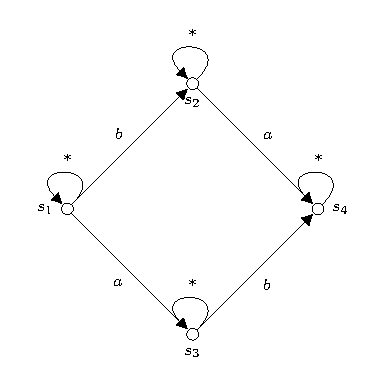
\includegraphics[scale=1.5]{Figures/2.Models-for-concurrency/idle-transition-system.pdf}
   %     \caption{A idle transition system}
   %     \label{fig:idle-transition-system}
   % \end{figure}
    
    
  %  Transition systems are made into a category by defining morphisms to be a simulation \cite{winskel95modelsCategory}. The idea is that a transition system $T$ simulates a transition system $T'$ if as soon as $T'$ can fire some action $e$ in some context, then $T$ can fire $e$ as well in some related context. A morphism $f: $T$ \rightarrow $T'$ $ defines the way states and transition of $T'$ are related to states and transitions of T. We introduce morphisms of transition systems as shown in \cite{winskel95modelsCategory}.
    
   % \begin{definition}[morphism of transition systems]\label{def:morphism-of-transition-system}
    %    A morphism from one transition system, T, to another, $T'$ , will be a pair $(\sigma, \lambda)$ in which
    %    \begin{itemize}
    %        \item $\sigma$ is a function from the states of $T$ to those of $T'$ .
    %        \item $\lambda$ is a partial function from the labels of $T$ to those of $T'$ such that for any transition $s \xrightarrow{a} s'$ of $T$ if $\lambda(a)$ is defined, then $\sigma(s) \xrightarrow{\lambda(a)} \sigma(s')$ is a transition of $T'$ ; otherwise, if $\lambda(a)$ is undefined, then $\sigma(s) = \sigma(s')$.
   %     \end{itemize}
   % \end{definition}
    
   
    
    %We write TS for the category of transition systems. Also, we name $TS_{A}$ its subcategory where we restrict to transition systems labeled on an alphabet A. The notion of transition systems and of morphisms between them is clearly related to (low dimensional) cubical sets / labeled directed graphs / labeled transition systems, but we will need to consider labeled cubical sets.
    
    %Transition systems are made into a category by defining morphisms to be some kind of simulation \cite{winskel95modelsCategory}. The idea is that a transition system $T_{1}$ simulates a transition system $T_{0}$ if as soon as $T_{0}$ can fire some action $a$ in some context, then $T_{1}$ can fire $a$ as well in some related context. A morphism $f: T_{0} \rightarrow T_{1}$ defines the way states and transition of $T_{0}$ are related to states and transitions of $T_{1}$.

   % In the above, we have used the notation L to stand for the set of events and the set of labels for those events. It is sometimes useful to make a distinction between the events themselves and their labels and to explicitly give a labelling as a function. This is important, for instance, in treating ‘\emph{relabelling}’ which leads to categorical fibrational situations (see the paper by Winskel and Nielsen, \cite{winskel95modelsCategory}). In order to make the distinction clearer, we will replace L by E and refer to its elements as ‘\emph{events}’ in what follows.
    
    % \begin{definition}[labeled transition system]\label{def:labeled-transition-system}
   %     A \emph{labeled} transition system consists of a transition system $T$ = (S, i, E, Tran) together with a set L of labels, and a function $l: E \rightarrow L$. We denote it by (T,L,l).
   % \end{definition}
    
   % \begin{definition}[Morphism of labeled transition systems]\label{def:labeled-transition-system}
   %     A morphism, ($\sigma,\tau, \lambda$) : ($T,L,l$) $\rightarrow$ ($T',L',l'$) between labeled transition systems consists of a morphism ($\sigma, \tau$):$T \rightarrow $T'$ $ between the underlying transition systems together with a partial function $\lambda : L \rightarrow L'$ such that $l' \circ \tau = \lambda \circ l$.
  % \end{definition}
    
   % For the sake of simplicity, we will not use these extensions to labeled transition systems or morphisms of labeled transition systems, though we will make an attempt to relate them in Chapter \ref{chap:Relationship with other models of concurrency}. We write LTS for the category of labeled transition systems.

%    One of the aspects of the classification of concurrent models of \cite{winskel94RelationshipsConcurrency} deals with concurrency, directly. \emph{Interleaving} models are known to be concurrent models that simulate concurrency whereas \emph{non-interleaving} or \emph{truly concurrent} models are able to distinguish concurrent execution from simulation on a one processor machine. In transition systems, one can simulate the parallel execution of two actions \emph{a} and \emph{b} as the \emph{interleaving} of \emph{a} then \emph{b} or \emph{b} then \emph{a} (see Figure \ref{fig:interleaving_square}). By design, interleaving models rely on the notion of \emph{atomic} actions and they are considered to be \emph{indivisible}, which makes them unsatisfactory for practical use where we would need to abstract away processes from unnecessary detail first, and then refine the semantics when we require more precision. Interleaving models are compelled to detail every part of a program execution \cite{?}. Moreover, interleaving models are not suited for giving semantics to most distributed programs since equating all the possible executions with some linear ordering of atomic actions means imposing a global clock as a ruler of the system. Finally, no possible discussion of the allocation of processes on the processors is possible since all executions in the interleaving approach are equivalent to some execution on a one processor machine.
    
    %The answer to this last problem is not quite given by all truly concurrent methods as we will show in Chapter 3. We really have to define a \emph{level of parallelism} as well as a \emph{level of mutual exclusion}. We propose here to refine this third axis in the classification of Winskel et al. \cite{winskel94RelationshipsConcurrency} into a real "\emph{level of parallelism/level of mutual exclusion}" axis. Let us first review some of the truly concurrent transition systems.
    
   % \ctlong{We may consider a few standard examples to also show a few problems which will be solved in the next chapters by non-interleaving models. May want to introduce the 3D cube here. Where the interleaving is the skeleton of the cube, as in nodes and edges only.}
    
  %  \ctlong{Examples such as Swiss flag, Dining philosophers, etc.}
    
    %%%% Part of introduction added here. Link it up!
  %  Traditionally, in a sequential program we would look at each of the possible executions of the program. When it comes to concurrency in practice, this becomes not feasible since the number of executions, or schedules, may grow exponentially with the size of the program. This is most commonly known as the \emph{state explosion problem}. Fortunately, it can be observed that many of the schedules are equivalent in the sense that one can be obtained from the other by permuting independent instructions: such equivalent executions will always lead to the same result. Hence, if one of those executions can be shown not to lead to an error, neither will any other execution which is equivalent to it.
    
  %  Sequential behaviour synchronizes the evolution of time and information. With concurrent behaviour time and information evolve more independently.
    
  %  This suggests that a model for concurrent programs should incorporate not only the possible executions of the program, as in traditional interleaving semantics, but also the commutations between instructions. Following the principle of what is now called \emph{true concurrency}. This principle is first presented in Section \ref{sec:asynchronous-transition-systems} and will be discussed in further detail in Chapter \ref{chap:An introduction to models for true concurrency}.
    
  %  We want to have a view that organizes states and events into two complementary spaces, state spaces or \emph{automata} and event spaces or \emph{schedules}, whose distances are respectively information deltas and time deltas. We will consider the relationship between these spaces as the \emph{state-event duality} described by Pratt in \cite{Pratt02eventStateDuality}. It was shown that the event structures from \cite{NielsenPW81eventstructures}, interpreted as schedules, were by design a model of \emph{true concurrency}, their dual prime algebraic domains were unmistakably automata of the "false concurrency" kind, with Figure \ref{fig:interleaving_square} a case in point having \{00, 01, 10, 11\} as its family of configurations. A perfect duality between true and false models of concurrency is paradoxical: for this distinction to be meaningful there must be something missing from the interpretation of prime algebraic domains as conventional automata. Leading to the investigation of non-interleaving models of concurrency, which will be review in the next chapter.
    
    
  %  One of the aspects of the classification of concurrent models of \cite{winskel94RelationshipsConcurrency} deals directly with concurrency. Some models are only simulating concurrency and are called $interleaving$ models whereas others distinguish concurrent executions from simulations on a one processor machine and are called \emph{non-interleaving} or \emph{truly concurrent} models. In transition systems, one can simulate the parallel execution of two actions $a$ and $b$ as the "interleaving" a then b or b then a (see Figure \ref{fig:interleaving_square}). Interleaving models rely on the notion of $indivisible$ or $atomic$ actions, which makes them unsatisfactory for practical use where we would like to be able to abstract away processes from unnecessary details first, and then refine the semantics when we ask for more precision. Interleaving models are compelled to detail every part of a program execution \cite{?}. Moreover, interleaving models are not suited for giving semantics to most distributed programs since equating all the possible executions with some linear ordering of atomic actions means imposing a global clock as a ruler of the system. Finally, no possible discussion of the allocation of processes on the processors is possible since all executions in the interleaving approach are equivalent to some execution on a one processor machine.
    
   % The answer to this last problem is not quite given by all truly concurrent methods as we will show in Chapter 3. We really have to define a \emph{level of parallelism} as well as a \emph{level of mutual exclusion}. We propose here to refine this third axis in the classification of Winskel et al. \cite{winskel94RelationshipsConcurrency} into a real "\emph{level of parallelism/level of mutual exclusion}" axis. Let us first review some of the truly concurrent transition systems.